\documentclass[12pt]{article}
\usepackage[a4paper, total={7.5in, 11in}]{geometry}
%\usepackage{array}
\usepackage{graphicx, subfig, wrapfig, fancyhdr, lastpage, multicol ,color,arydshln,makecell}
\newcommand\headerMe[2]{\noindent{}#1\hfill#2}
\usepackage[mathscr]{euscript}
\usepackage{tabularray}

\setlength{\columnseprule}{1pt}
\def\columnseprulecolor{\color{blue}}


\pagestyle{fancy}
\fancyhf{}

\cfoot{ \vspace{-0.8cm}\em{Page \thepage \hspace{1pt} / \pageref{LastPage}}}
\begin{document}

\headerMe{Royaume du Maroc}{année scolaire \emph{2022-2023}}\\
\headerMe{Ministère de l'Éducation nationale, }{  Professeur :\emph{Zakaria Haouzan}}\\
\headerMe{du Préscolaire et des Sports}{Établissement : \emph{Lycée SKHOR qualifiant}}\\
%\vspace{-1cm}
\begin{center}
Devoir Surveillé  N°2 \\
    2ème année baccalauréat Sciences physiques\\
Durée 2h00
\\
    \vspace{.2cm}
\hrulefill
\Large{Chimie 7pts - 45min}
\hrulefill\\

    \emph{Les deux parties sont indépendantes}
\end{center}
%end Headerss------------------------
%__________________Chimie ______________________-
%%%%%%%+_+_+_+_+_+_+_+_+_Partie1

 \section*{Transformations non totales d'un système chimique\dotfill(7pts)-45min }
%\begin{wrapfigure}{r}{0.16\textwidth}
	%\vspace{-1.2cm}
%%\begin{center}
  %%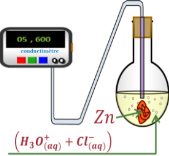
\includegraphics[width=0.16\textwidth]{./img/chimie01.png}
%%\end{center}
%\end{wrapfigure}


%\begin{wrapfigure}[1]{r}{0.5\textwidth}
	%\vspace{0.5cm}
%\begin{center}
  %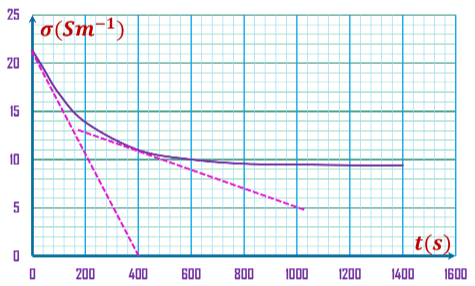
\includegraphics[width=0.5\textwidth]{./img/chimie02.png}
%\end{center}
%\end{wrapfigure}

 \section*{Partie 1 : la dissolution de l’acide éthanoïque dans l’eau.
}

	On dispose de deux solutions (S1) et (S2) d’acide éthanoïque $CH_3COOH$.

	La conductivité de la solution (S1) de concentration molaire $C_1=5.10^{-2}mol/L$ ; $\sigma_1= 3,5.10^{-2}S/m$.

	La conductivité de la solution (S2) de concentration molaire $C_2=5.10^{-3}mol/L$ ; $\sigma_2=1,1.10^{-2}S/m$.

	On considère que la dissolution de l’acide éthanoïque dans l’eau est limitée.


	\begin{tabular}{c|l}
		1 & \makecell[l]{\textbf{1. }Ecrire l’équation modélisant la dissolution de l’acide éthanoïque dans l’eau.}\\

		1 & \makecell[l]{\textbf{2. }Trouver l’expression de la concentration molaire effective $[H_3O^+]_{(eq)}$ des ions oxoniums à \\l’équilibre en
		fonction de $\sigma$ et $\lambda_{CH_3COO^-}$ et $\lambda_{H_3O^+}$.}\\

			1 & \makecell[l]{\textbf{3. }Calculer $[H_3O^+]_{(eq)}$ dans chacune des solutions (S1) et (S2).}\\

			1 & \makecell[l]{\textbf{4. }Déterminer les taux d’avancement final $\tau_1$ et $\tau_2$ de la réaction de l’acide éthanoïque avec l’eau\\dans chacune
des solutions (S1) et (S2). \\Déduire l’influence de la concentration initiale de la solution sur le taux
d’avancement final.}
			\end{tabular}

	Les conductivités molaires ioniques : $\lambda_{H_3O^+}$=$3,49.10^{-2}S.m^2/mol$ ; $\lambda_{CH_3COO^-}$=$4,09.10^{-3}S.m^2/mol$


\section*{Partie 2 : L'acide propanoïque }

L'acide propanoïque $C_2H_5COOH$ est un acide gras, utilisé dans la synthèse de certains produits organiques et
pharmaceutiques, de parfums et dans la médecine vétérinaire.

On considère, à 25°C, une solution aqueuse (S) d’acide propanoïque de concentration molaire \\$C $=$2,0.10^{-3}mol.L^{-1}$ et de volume $V $=$1,0 L$. La mesure de la conductivité $\sigma$ de la solution (S) a donné la valeur $\sigma = 6,2.10^{-3} S.m^{-1}$.

$$\lambda_{H_3O^+} = 35.10^{-3}S.m^2/mol \hspace{1cm} \lambda_{C_2H_5COO^-}=3,58.10^{-3}S.m^2/mol$$






\begin{tabular}{c|l}
	1  & \makecell[l]{ \textbf{1. }Écrire l’équation chimique modélisant la réaction de l’acide propanoïque avec l’eau.}\\

	1	 & \makecell[l]{\textbf{2. }Dresser le tableau d’avancement de la réaction en utilisant les grandeurs $C_A$, $V_A$,\\l'avancement $x$ et l'avancement $x_{eq}$ à l'état d’équilibre du système chimique.\\ Déterminer la valeur de l'avancement maximal.}\\

	1 & \makecell[l]{\textbf{3. }Vérifier que la valeur de l'avancement à l'état d’équilibre est $x_{eq} = 1, 6.10^{-4} mol$.}\\

	1 & \makecell[l]{\textbf{4. }Calculer la valeur du taux d'avancement final.}\\
\end{tabular}


 On considère une solution aqueuse (S') d'acide propanoïque de concentration molaire $C_A'$=$2.10^{-4} mol.L^{-1}$ et de
$pH = 4, 3$ . On note $\tau'$ le taux d'avancement final de la réaction de l'acide propanoïque avec l'eau dans ce cas.

\begin{tabular}{c|l}
	1 & \makecell[l]{\textbf{5. }Déterminer la valeur de $\tau'$.}\\

	1 & \makecell[l]{\textbf{6. }Comparer les valeurs de $\tau$ et $\tau'$ . Déduire.}

\end{tabular}









%\hrulefill
%\Large{Physique 13pts/78min}
%\hrulefill\\
\newpage
\begin{center}
    %\vspace{.60cm}
\hrulefill
\Large{Physique 13pts - 75min}
\hrulefill\\
    \emph{Les  parties sont indépendantes}
\end{center}

%\vspace{-1cm}
\section*{Partie 1 : La radioactivité au service de la médecine\dotfill(4pts)}

%\begin{wrapfigure}[2]{r}{0.19\textwidth}
  %\begin{center}
	  %\vspace{-2cm}
	%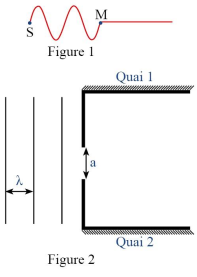
\includegraphics[width=0.19\textwidth]{./img/ex6.png}
  %\end{center}
%\end{wrapfigure}

La médecine est l’un des domaines qui a connu l’application de la radioactivité en utilisant des noyaux
radioactifs pour diagnostiquer et traité des maladies, l’un des noyaux utilisés est le rhénium 186 dans
le but de soulager les malades atteints de polyarthrite rhumatoïde

Les données : La constante radioactive du rhénium $_{75}^{186}Re$ est $\lambda = 2,2.10^{-6}s^{-1}= 0,19jour^{-1}$

\textbf{1. La désintégration d’un noyau de rhénium $_{75}^{186}Re$.}

\begin{tabular}{c|l}

	1 & \makecell[l]{\textbf{1.1 }Donner la composition du noyau du rhénium $_{75}^{186}Re$.}\\

	1 & \makecell[l]{\textbf{1.2 }La désintégration du noyau de rhénium $_{75}^{186}Re$ donne un noyau d’osmium $_{76}^{186}Os$.\\
Ecrire
l’équation de désintégration du rhénium et déterminer la nature de cette désintégration}\\
	\end{tabular}

	\vspace{0.5cm}
\textbf{2. Injection locale d’une solution contenant du rhénium 186.
Le produit injectable se présente sous la forme d’une solution contenue dans un flacon de volume $V_0= 10 mL$ ayant une activité $a_0 = 4.10^9Bq$ à la date $t=0$, c'est-à-dire à la sortie du laboratoire pharmaceutique.}
	\begin{tabular}{c|l}

		1 & \makecell[l]{\textbf{2.1 }Déterminer en jours la valeur de demi-vie $t_{1/2}$ du rhénium $_{75}^{186}Re$}\\

		0,5 & \makecell[l]{\textbf{2.2 }Trouver, à l’instant $t_1 = 4,8jours$, le nombre $N_1$ de noyau de rhénium contenu dans le flacon.}\\

		0,5 & \makecell[l]{\textbf{3.2 } À l’instant $t_1$ on prélève du flacon de volume $V_0 = 10mL$ une injection de volume V contenant \\$N = 3,65.10^{13}$ noyaux de rhénium 186, on l’injecte à un malade dans l’articulation de l’épaule, \\trouver la valeur de V.}\\
	\end{tabular}


\section*{Partie 2 :  Centrale nucléaire \dotfill(9pts)}
Dans une centrale nucléaire, les noyaux d'uranium $^{235}_{92}U$ subissent la fission sous le choc d'un neutron
lent. Un des nombreux processus possibles conduit à la formation d'un noyau de lanthane $^{144}_{57}La$ ,d'un noyau de brome $^{88}_{35}Br$ et  de plusieurs neutrons.

\begin{tabular}{c|l}

 1& \makecell[l]{\textbf{1. } Définissez l'énergie de liaison d'un noyau.}\\

 1 & \makecell[l]{\textbf{2. } Donnez l'expression littérale qui permettra son calcul.}\\

 1 & \makecell[l]{\textbf{3. } Calculez, en MeV, l'énergie de liaison d’un noyau $^{235}_{92}U$.}\\

 1 & \makecell[l]{\textbf{4. } Calculez l’énergie de liaison par nucléon de ce noyau.}\\

 1 & \makecell[l]{\textbf{5. } Ecrivez l’équation de la réaction de fission étudiée.}\\

 1 & \makecell[l]{\textbf{6. } Exprimez l'énergie libérée par la fission d'un noyau $^{235}_{92}U$ en fonction des énergies de liaison par
\\ nucléon du noyau père et des noyaux fils et calculez la valeur de cette énergie en MeV.}

 \end{tabular}

\textbf{7.  Dans le cœur de la centrale, de nombreuses autres réactions de fission du noyau $^{235}_{92}U$ se produisent. La perte de masse est, en moyenne, de 0,200 u par noyau.}


\begin{tabular}{c|l}

	1,5 & \makecell[l]{\textbf{7.1. } Calculez, en MeV, l'énergie moyenne libérée par la fission d’un noyau. Ce résultat est-il \\en concordance avec celui de la question 6 ?}\\

	1,5 &\makecell[l]{\textbf{7.2. }Calculez, en joule, l'énergie moyenne libérée par une mole de noyaux $^{235}_{92}U$ } 

\end{tabular}

\textbf{Données :}
\begin{itemize}
	\item Célérité de la lumière dans le vide : $c = 2,998 . 10^8 m.s^{-1}$  
	\item Masse du noyau d’uranium 235 : $m( ^{235}_{92}U) = 235,0134u$ 

	\item Energies de liaison par nucléon : $E_l/A(^{144}_{57}La) = 8,28MeV/nucl$éon  ; $E_l/A(^{88}_{35}Br)$=$8,56MeV/nucl$éon
	\item Constante d'Avogadro : $N_A = 6,02.10^{23} mol^{-1}$
	\item $1u$ = $1,66055.10^{-27}Kg$ et $1eV = 1,602.10^{-19}J$
	\item Masse d’un proton : $m(^1_1p) = 1,0073u$ ; Masse d’un neutron $m(^1_0n) = 1,0087u$
\end{itemize}





\end{document}
